\section{Bài 3: Traceroute}
Nếu bạn dùng Window thì dùng lệnh \textbf{\textit{tracert}}, nếu bạn dùng Linux/iOS thì bạn dùng lệnh \textbf{\textit{traceroute}}. Lưu ý kết quả bắt gói tin trên Window và Linux/iOS sẽ khác nhau, vì vậy câu trả lời phụ thuộc bạn dùng OS nào.\\
Bật wireshark để bắt gói tin lệnh traceroute từ máy của mình (có thể dùng máy ảo) đến \textbf{\textit{www.fit.hcmus.edu.vn}} (FIT). \\
Bài tập được thực hiện trên máy tính sử dụng hệ điều hành \textbf{Windows 11}.\\
Kết quả bắt gói tin chi tiết được lưu trong tập tin \textbf{bai3.pcapng}.\\

\textbf{1. Chụp hình kết quả bắt gói tin sau khi traceroute hoặc tracert (thấy được những gói tin liên quan).}\\
Kết quả bắt gói tin sau khi tracert như sau.
\begin{figure}[H]
\begin{center}
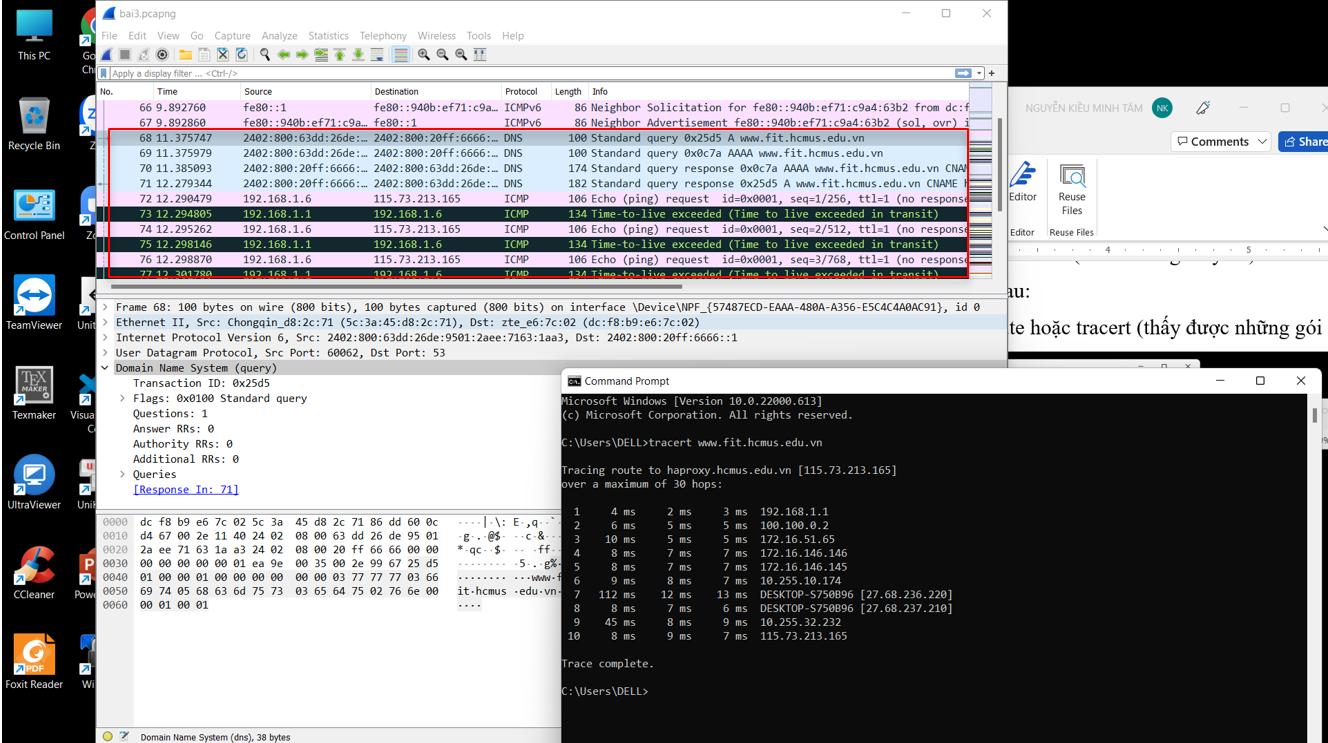
\includegraphics[scale=1]{../figures/p3/p3_res1}
\end{center}
\caption{Kết quả bắt gói tin sau khi tracert}
\end{figure}
Các gói tin được bắt tính từ lệnh tracert được thể hiện ở phần đóng khung màu đỏ trên hình vẽ. Đó là các gói tin đầu tiên bắt đầu từ khi tracert (gói tin số 68).

\textbf{2. Cho biết traceroute/tracert dùng để làm gì?}\\
Traceroute/tracert dùng để xác định vết đường đi của gói tin giữa hai host: source host và destination host. 
Thông tin này được thể hiện qua các gói tin ICMP (gói tin IP có trường protocol = 1). Và dựa vào thông tin tương ứng trên các trường của thông điệp ICMP, host nguồn xác định được địa chỉ IP của các router trên đường truyền. \supercite{slides, cn}

\textbf{3.	Cho biết địa chỉ IP của máy gửi request.}\\
Địa chỉ IP của máy gửi request là 192.168.1.6.
\begin{figure}[H]
\begin{center}
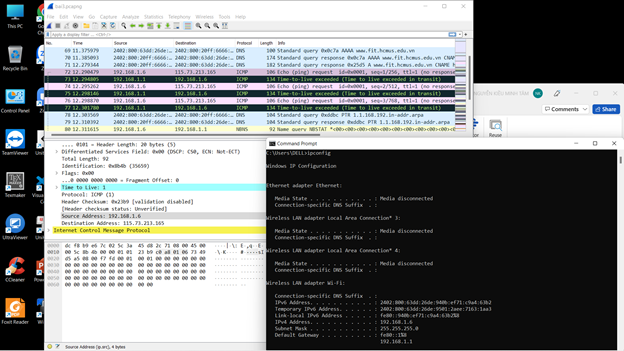
\includegraphics[scale=1]{../figures/p3/p3_hostip}
\end{center}
\caption{Địa chỉ IP của máy gửi request}
\end{figure}

\textbf{4.	Cho biết cách máy tính xác định được địa chỉ IP của FIT.}\\
Máy tính sẽ gửi gói tin DNS query lên DNS server để “hỏi”, sau đó DNS Server sẽ trả lời qua gói tin DNS response. 
\begin{itemize}
\item Gói tin DNS query được gửi từ destination host là gói tin số 68 (được lưu trong file \textbf{bai3.pcapng}).
\begin{figure}[H]
\begin{center}
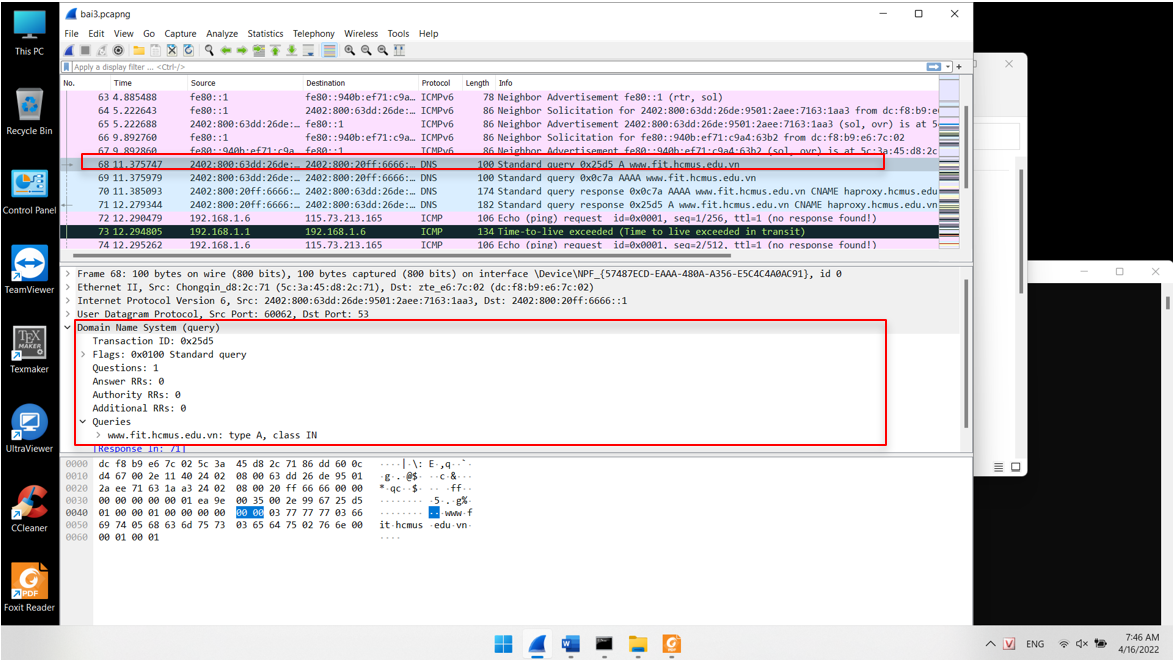
\includegraphics[scale=1]{../figures/p3/p3_dns1}
\end{center}
\caption{Gói tin DNS query}
\end{figure}
\item Và gói tin trả lời tương ứng là gói tin số 71 (được lưu trong file \textbf{bai3.pcapng}). Hình vẽ cho thấy có FIT có 3 địa chỉ IP 115.73.213.165, 14.161.23.204, 14.241.254.131. Trong lần này traceroute được thực hiện tới địa chỉ IP 115.73.213.165. 
\begin{figure}[H]
\begin{center}
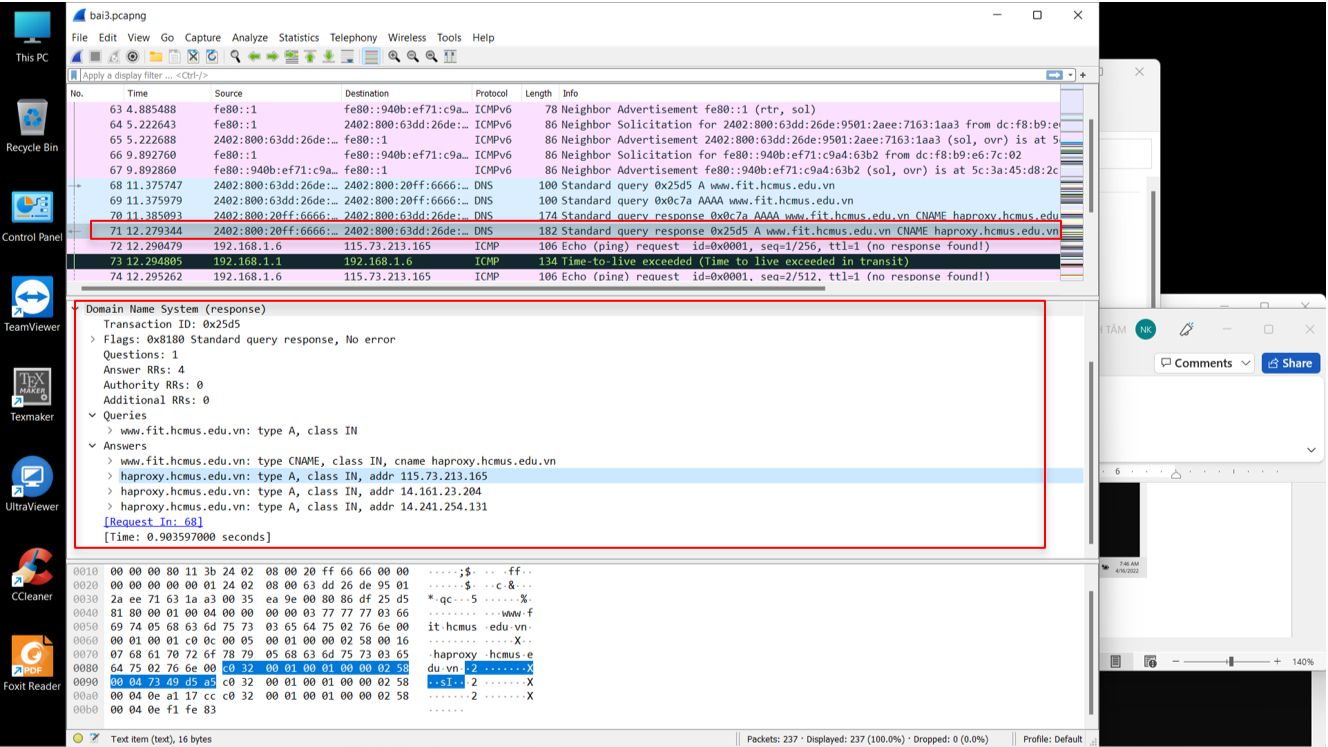
\includegraphics[scale=1]{../figures/p3/p3_dns2}
\end{center}
\caption{Gói tin DNS query response}
\end{figure}
\end{itemize}
